\chapter{Filtered BioRED Annotation Guidelines Used For Prompting}
\label{app:filtered_biored_guidelines}
\begin{lstlisting}
## Guideline of the entities

### General rules
- Annotate all the spans of all the six concept types.
- The full text can be accessed to clarify the concept spans and identifiers.
- The abbreviation and its long form should be annotated separately if possible. prostaglandin E2 (PGE2) in the text, "prostaglandin E2" and "PGE2" should be both annotated to chemicals with the same identifier (D015232).
- Annotate both the full name and abbreviation in one entity, if the boundary of the entity covers both of them. For instance, annotate "Deoxyguanosine kinase (dGK) deficiency" entirely to a disease (PMID:19394258).
- Annotate the composite entity spans (e.g., "MMP-1, -2") entirely. The identifiers of the multiple concepts should
be entered separated by "," with no space (e.g., "4312,4313").
- Annotate any concept identifier span (e.g., "OMIM 307800" and "rs729302").
- Annotate the concept spans with misspelling ("HLRRC" in PMID:18366737).

### Gene
- The gene spans should be linked to NCBI Gene ID (https://www.ncbi.nlm.nih.gov/gene/). Specify the corresponding species and the identifiers to the gene spans.
- Annotate the gene families including paralogs/orthologs (e.g., bone morphogenetic protein(bmp)), but DO NOT annotate the functional based families (e.g., tumor suppressor gene, protein kinase).
- Following the previous rule, if at least one of the gene family members mentioned in the text, the identifiers of those members are assigned to the family name (e.g., in "Cytochrome P-450 genes (CYP1A1, CYP2A6, CYP2D6, and CYP2E1)", Cytochrome P-450 genes should be assigned with NCBI Gene: 1543,1548,1565,1571). If no family member is in the text, the first gene reached in the gene family should be assigned (e.g., matrix metalloproteinases to NCBI Gene:4312(MMP1)).
- In experimental studies, annotate the gene identifier corresponding to the organism/species that is the source of the
gene (for example mouse gene transfected into human cells is annotated to record for mouse gene).
- DO NOT annotate the genes, if they are named for cells and pathways.

### Disease
- The diseases refer to MEDIC which is a combination of MESH (https://meshb.nlm.nih.gov/search) and OMIM (https://omim.org/). We annotate the MESH identifier, if a disease has both the MESH and OMIM identifiers.
- If no specific disease concept can be reached in MEDIC by the annotated span, we annotate the closest hypernym concept that logically describes the disease span(e.g., X-linked retinitis pigmentosa to D012174 (retinitis pigmentosa) in PMID:17935240). Otherwise, "-" is assigned to the mismatched diseases.
- Annotate the diseased-related phenotypes but not other (e.g., short ear in PMID:17345627).
- DO NOT annotate the high-level diseases (e.g., "genetic disorder").
Excludes:
- Cis-acting disease (PMID:12442272)
- genetic disorders (PMID:18046082)
- familial disorder (PMID:20806042)
- Annotate "drug addiction" to "disease".
- Annotate the symptoms to diseases.
- DO NOT annotate overdose.
- DO NOT annotate the mental status and phenotypes to diseases unless the term is exactly recorded in MEDIC. e.g., decline in sympathetic tone (PMID:19067809)
- DO NOT annotate references to biological processes such as "tumorigenesis" or "cancerogenesis".
- Annotate minimum necessary text spans for a disease. For example, select "hypertension" instead of "sustained hypertension.", unless the span covers the prefix or the suffix can exactly match a specific concept identifier (e.g., "chronic bronchitis" to D029481).

### Chemical
- Chemical spans should be linked to MESH (https://meshb.nlm.nih.gov/search). "-" is assigned to the mismatched chemicals.
- Annotate the chemical abbreviation with the dose. For example "In addition, GABA content of mice hippocampus treated with GFC75 plus P400 showed an increase of 46.90% when compared with seized mice.", 75 and 400 suffixes are the doses. In this case, we annotate GFC75 and P400 as chemical spans. (PMID:24911645).
- Annotate the chemical resource for extracts, e.g., "ethanolic extract of Daucus carota seeds (DCE)" in PMID:16755009; "grape seed proanthocyanidin extract" in PMID:11334364.
- DO NOT annotate antibodies to chemicals. (PMID:17595233) (PMID:20648600)
- DO NOT annotate saline, placebo, water, and juice.
- DO NOT annotate residue, free radicals.
- DO NOT annotate staining chemical (e.g., hematoxylin in PMID:24442316)
- DO NOT annotate vaccines.

### Species
- The species spans should be linked to NCBI Taxonomy ID (https://www.ncbi.nlm.nih.gov/taxonomy/)
- DO NOT annotate beyond species rank (e.g., annotate homo sapiens but do not annotate mammalian which is a taxonomy class)

### Variant
- The annotation of the variants follows tmVar annotation guidelines, the variants should be linked to dbSNP (https://www.ncbi.nlm.nih.gov/snp) accession number (RS#) when possible. Otherwise, we annotate the variant components (e.g., wild type, location, and mutant) following the tmVar component format (e.g., V600E to "p|SUB|V|600|E").
- DO NOT annotate residue of the gene modification.
- For those variants that cannot be normalized: In our observations on the variant recognition/normalization dataset, around 50-60% of the variants cannot be normalized to the specific concept identifiers in dbSNP. For those, we enumerate the components of the variants.

### Normalized components of the curated variant types:

#### Variant on DNA Sequence
Example(s) and normalized component or identifier(s):
- c.1922G>A: c|SUB|G|1922|A
- C-to-G transition was identified at nucleotide 857: c|SUB|C|857|G

#### Variant on protein sequence
Example(s) and normalized component or identifier(s):
- R114H: p|SUB|R|114|H
- methionine to threonine substitution at codon 235: p|SUB|M|235|T

#### RS number
Example(s) and normalized component or identifier(s):
- rs763780: rs763780

#### Allele on DNA sequence
Example(s) and normalized component or identifier(s):
- -281G: c|Allele|G|-218

#### Allele on protein sequence
Example(s) and normalized component or identifier(s):
- L638: p|Allele|L|638
- stop codon at position 372: p|Allele|X|372

#### Nucleotide or acid change
Example(s) and normalized component or identifier(s):
- G > C: c|SUB|G||C
- valine for glutamate: p|SUB|V||E

## Guideline of the relation pairs

### General rules
- We only annotate the (1) Popular associations and the (2) Corresponding gene/species in Figure 1.
- Co-occurrence in the same sentence is not required.
- DO NOT annotate a confirmed irrelevance. (e.g., "Nonetheless, NBS1 gene heterozygosity is not a major risk
factor for lymphoid malignancies in childhood and adolescence" in PMID:16152606)
- Annotate the associations with explicit statements in the text.
- The full text is NOT allowed to access. DO NOT annotate if the statement in the abstract is not clear. (e.g.,
PMID:14722929)
- For Co-treatment, we annotate "Negative_Correlation" between the two chemicals and the disease, and a
"Cotreatment" relation between the two chemicals. For an example in PMID:16720068, "Possible neuroleptic
malignant syndrome related to concomitant treatment with paroxetine and alprazolam.".
- For Drug_Interaction, we annotate "Positive_Correlation" between the two chemicals and the disease, and a
"Drug_Interaction" relation between the two chemicals.

### Disease-chemical
- Annotate the association of chemicals and disease due to the "toxicity" and "drug-induced", but not annotate the
chemicals with the disease concept-"toxicity" directly.
    -  PMID:19728177
    "RESULTS: Our patient was admitted to the MICU after being found unresponsive with presumed toxicity from acetaminophen which was ingested over a 2-day period. ... In patients with FHF and cerebral edema from acetaminophen overdose, prolonged therapeutic hypothermia could potentially be used as a life saving therapy and a bridge to hepatic and neurological recovery." We annotate the associations between acetaminophen and FHF/cerebral edema due to the toxicity, but we do not annotate acetaminophen and toxicity.
- Annotate the relation between the target disease and the measure level of the molecules/chemicals in blood test
with correlation, "Compared with control patients, CRF and ESRD patients had higher preoperative serum
creatinine levels, a greater percentage of patients with hepatorenal syndrome.", the pairs of "CRF, creatinine" and
"ESRD, creatinine" is annotated. (PMID:11773892)
- DO NOT annotate the association of disease to the staining chemicals. For instance, "The extent of neuronal injury
was determined by 2,3,5-triphenyltetrazolium staining." (PMID:1711760) and "Renal lesions were analyzed in
hematoxylin and eosin, periodic acid-Schiff, and Masson's trichrome stains. SRL-treated rats presented proteinuria
and NGAL (serum and urinary) as the best" (PMID:24971338)
- DO NOT annotate the association of any disease with the chemical concept "analgesia" in "patient-controlled
analgesia (PCA) pump". For instance, "patient-controlled analgesia (PCA) pump" (PMID:9672936)
- DO NOT annotate toxicity with its chemical. For instance, do not annotate "unresponsive with presumed toxicity
from acetaminophen" (PMID:19728177)
- Annotate the chemicals which prevents the chemical-induced disease (PMID:24971338+18503483)

### Disease-gene
- DO NOT annotate the prognostic factor of genes or its variants to the target disease.
- Annotate the negative correlation (e.g., knockdown gene to the target disease). For instance, annotates Gankyrin
and HCC in "Gankyrin expression in the tumor microenvironment is negatively correlated with progression-free
survival in patients undergoing sorafenib treatment for HCC." (PMID:28777492)
- DO NOT annotate the symptoms of the target disease to the correlated variants or genes, unless the clear statement
between the symptom and variant is provided.

### Disease-variant & Disease-gene
- Annotate the corresponding diseases with the variant when it is observed in patients.
- Annotate the diseases with the associated genes.
- Annotate the corresponding gene of the variant with the variant-associated disease.
- Annotate the association between the variants (and corresponding gene) and the diseases belonging to the target
disease. For instance, annotate the association between "autosomal recessive disease" and "272gly----stop"
(PMID:1671881).
- Annotate the minor association (e.g., the observation of the association on few patients).
- Annotate the associations in the particular races.
- Annotate the association between disease and variant if the inheritance of the genetic disease is confirmed by the
variant.
- DO NOT annotate the symptoms of the target disease to the correlated variants or genes, unless the clear statement
between the symptom and variant is provided. (ex in PMID: 1952108)

### Gene-gene
- Annotate the pairs of the members in the protein complex, e.g., EPO/EPOR (PMID:22808010).
    - In "We cloned the cDNA of three remaining human NADH:ubiquinone oxidoreductase subunits of this IP fraction: the NDUFS2 (49 kDa), NDUFS3 (30 kDa), and NDUFS6 (13 kDa) subunits.", all the pairs between two of the NDUFS2, NDUFS3, and NDUFS6 are annotated. (PMID:9647766)
- DO NOT annotate the "is_a" association between two genes. For instance, DO NOT annotate "breast and ovarian
cancer gene" and "BRCA1" (PMID:8944024).
- Annotate protein-protein interaction for singling proteins and the receptors. For instance, "Epo-R signaling
proteins (Akt, STAT5, p70s6k, LYN, and p38MAPK)" (PMID:27640183)

### Gene-chemical
- Annotate the chemical with the gene receptor. For instance, "antipsychotic drugs that have a high affinity with the
D2 receptor" (PMID:16867246)

### Chemical-chemical
- DO NOT annotate the "is_a" association between two chemicals. For instance, "Nefiracetam is a novel
pyrrolidone derivative" (PMID:8829135)
- Annotate the chemical-chemical association for the chemical contributes to the other for treatment, side effects and
drug-drug interaction. In "the midline serotonin B3 cells in the medulla contribute to the hypotensive action of
methyldopa", the pair of serotonin and methyldopa is annotated. (PMID:2422478)

### Chemical-variant
- Annotate the chemical with the variant, if the chemical binding ability of the gene impaired by the variant. For
instance, "This variant (apoE Guangzhou) may cause a marked molecular conformational change of the apoE and
thus impair its binding ability to lipids." (PMID:18046082)
- Annotate the chemical with the variant, if different mRNA stability between different alleles affected by the
chemical. For instance, "After transfection and inhibition of transcription with actinomycin D, analysis of mRNA
turnover failed to reveal differences in mRNA stability between A118 and G118 alleles, indicating a defect in
transcription or mRNA maturation." (PMID:16046395)

### Others
- DO NOT annotate the pairs of concepts with negative conclusions (e.g., "not significant", "no correlation was
observed"). For instance, "For most of the variants identified in the Kenyan and Sudanese study population, a
causative association with NSARD appears to be unlikely" is not annotated.
- In the case that a disease is induced by a chemical, and the other concepts (e.g., chemical, or protein) treats/affects
the induced disease, we annotate the three pairs by following examples. For instance:
    -  "In addition, there is convincing clinical evidence that monotherapy with continuous subcutaneous apomorphine infusions is associated with marked reductions of preexisting levodopa-induced dyskinesias." (PMID:11009181)
        - Positive_Correlation between levodopa and dyskinesias
        - Negative_Correlation between apomorphine and dyskinesias
        - Negative_Correlation between apomorphine and levodopa
    - Absence of PKC-alpha attenuates lithium-induced nephrogenic diabetes insipidus. (PMID:25006961)
        - Positive_Correlation between lithiumand nephrogenic diabetes
        - Positive_Correlation between PKC-alpha and dyskinesias
        - Positive_Correlation between PKC-alpha and lithium
    - Characterization of a novel BCHE "silent" allele: point mutation (p.Val204Asp) causes loss of activity and prolonged apnea with suxamethonium. (PMID:25054547)
        - Positive_Correlation between p.Val204Asp and apnea
        - Negative_Correlation between apnea and suxamethonium
        - Association between p.Val204Asp and suxamethonium
        - Association between BCHE and apnea
        - Association between BCHE and suxamethonium
    -  Curcumin prevents maleate-induced nephrotoxicity (PMID:25119790)
        - Negative_Correlation between Curcumin and nephrotoxicity
        - Positive_Correlation between maleate and nephrotoxicity
        - Negative_Correlation between Curcumin and maleate
- Annotate the previous reported association, even the conclusion demonstrates the association is not significant. (PMID:15824163)

### Guideline of the relation types
We collected a list of relation types between two concepts (e.g., upregulation between two genes). Further, we merged some of the relation types to narrow down the curation complexity and increase the number of instances in each relation type.

The following mappings define how directional relation types should be converted to the BioRED relation types.
**Gene <-> Gene**
| Directional relation | BioRED relation |
|----------------------|-----------------|
| Upregulation | Positive_Correlation |
| Downregulation | Negative_Correlation |
| Regulation | Association |
| Positive_Correlation | Positive_Correlation |
| Negative_Correlation | Negative_Correlation |
| Bind | Bind |
| Modification | Association |
| Association | Association |

**Chemical <-> Gene**
| Directional relation | BioRED relation |
|----------------------|-----------------|
| Exhibition (Chemical -> Gene) | Positive_Correlation |
| Response (Gene -> Chemical) | Positive_Correlation |
| Suppression (Chemical -> Gene) | Negative_Correlation |
| Resistance (Gene -> Chemical) | Negative_Correlation |
| Association | Association |
| Receptor | Bind |
| Chem_Modification | Association |

**Chemical <-> Variant**
| Directional relation | BioRED relation |
|----------------------|-----------------|
| Association | Association |
| Resistance | Negative_Correlation |
| Response (and sensitivity) | Positive_Correlation |

**Gene <-> Disease**
| Directional relation | BioRED relation |
|----------------------|-----------------|
| Positive_Correlation | Positive_Correlation |
| Negative_Correlation | Negative_Correlation |
| Association | Association |

**Variant <-> Disease**
| Directional relation | BioRED relation |
|----------------------|-----------------|
| Cause | Cause |
| Association | Association |

**Chemical <-> Disease**
| Directional relation | BioRED relation |
|----------------------|-----------------|
| Treatment | Negative_Correlation |
| Induce | Positive_Correlation |
| Association | Association |

**Chemical <-> Chemical**
| Directional relation | BioRED relation |
|----------------------|-----------------|
| Cotreatment | Cotreatment |
| Inhibition | Negative_Correlation |
| Increase | Positive_Correlation |
| Drug_Interaction | Drug_Interaction |
| Association | Association |
| Comparison | Comparison |

### Disease-chemical
- Positive_Correlation
    - Chemical-induced disease.
    - Chemical (or Higher dose of the chemical) causes a higher risk of the disease.
    - Disease causes the increase of the chemical measured level.
    - The level of the chemical and the risk of the disease present a positive correlation.
    - Chemical exposures during development alter disease susceptibility later in life.
- Negative_Correlation
    - The disease-treated chemical/drug.
    - Disease causes the decrease of the chemical measured level.
    - The chemical/drug drops down the susceptibility of the disease.
- Association
    - A safety drug of the potential disease (PMID:20722491 - capecitabine(C110904) - hepatic and renal dysfunctions(D008107|D007674))
    - The associations of the pairs which cannot be categorized to positive/negative correlation.
    - The associations without clear description.

### Disease-gene
- If an association between a variant and a disease is confirmed, the corresponding gene should associate with the disease by "Association" type.
- Positive_Correlation
    - The overdose of protein causes the disease.
    - The knockout gene prevents the disease.
    - The side effect of protein (drug) causes the disease
- Negative_Correlation
    - The protein (drug) is used to treat/prevent the disease.
    - Lack of the protein causes the disease.
    - The knockout gene causes the disease.
- Association
    - The associations of the pairs which cannot be categorized to previous relation types.
    - The associations without clear description.
    - The functional gene prevents the occurrence of the disease.
    - Protein deficiency.

### Disease-variant
- Positive_Correlation
    - The variant increases the risk of the disease.
    - Significant frequency (p-value) of the disease with the specific allele.
    - The variant causes the gene to be either over-express or non-functional and further causes disease (or raises the disease susceptibility).
    - Disease is caused by protein deficiency, and the variant is responsible for the deficiency.
    - The variant plays a role in genetic predisposition to the disease.
    - The variant has a significant contribution to the disease.
    - Annotate "Positive_Correlation" to the pair of "founder mutation" and the target disease. (PMID:10788334,19394258)
- Negative_Correlation
    - The variant decreases the risk of the disease.
- Association
    - The variant observed from a number of patients.
    - The variant is associated with a lower prevalence of the disease or is responsible for the lower disease susceptibility
    - The associations of the pairs which cannot be categorized to "Cause" relation type.
    - The associations without clear description.
### Gene-gene
- Positive_Correlation
    - Two genes present the positive correlation in gene expression results.
    - Gene A is a transcription factor of the gene B, and gene A upper regulates the gene B.
    - Two genes present a positive correlation in any way.
- Negative_Correlation
    - Two genes present the negative correlation in gene expression results.
    - Gene A is a transcription factor of the gene B, and gene A down regulates the gene B.
    - Two genes present a negative correlation in any way.
- Bind
    - physical interaction between two proteins.
    - Protein A binds the promoter of gene B.
    - Two or more proteins in a complex.
    - Annotate "bind" to the protein and its protein receptor. ("androgen receptor" and "androgen" in PMID:15599941)
    - If the binding causes a positive or negative correlation, annotate the association to Positive_Correlation/Negative_Correlation.
    - DO NOT annotate the protein bind on a gene promoter region.
- Association
    - Annotate the modification (e.g, phosphorylation, dephosphorylation, acetylation ,deacetylation and other modifications) to association.
    - The associations of the pairs which cannot be categorized to any other association types.
- The associations without clear description.

### Gene-chemical
- If an association between a variant and a chemical is confirmed, the same association type should be
assigned to the corresponding gene of the variant and the chemical.
    - Positive_Correlation
    - The chemical causes a higher expression of the gene.
    - Higher gene expression causes higher sensitivity of the chemical.
    - The variant triggers the chemical adverse effects or causes the side effect worse.
    - The gene causes the chemical over-response.
    - Two genes present a positive correlation in any way.
-  Negative_Correlation
    - The chemical causes a lower expression of the gene.
    - Higher gene expression causes lower sensitivity (resistance) of the chemical, and vise versa.
    - The variant has a protective role for the development of the chemical adverse effects.
    - The gene causes the chemical resistance.
    - Two genes present a negative correlation in any way.
- Association
    - The associations of the pairs which cannot be categorized to any other association types.
    - The associations without clear description.
- Bind
    - A chemical binds the promoter of a gene.
    - A protein is the chemical receptor.
    - If the binding causes a positive or negative correlation, annotate the association to Positive_Correlation/Negative_Correlation.

### Chemical-chemical
- Positive_Correlation (between A and B)
    - Chemical A increases the sensitivity of the chemical B.
    - Chemical A increases the treatment/inducing effectiveness of the chemical B to a disease.
    - Chemical A increases the effectiveness of the gene activation caused by chemical B.
- Negative_Correlation (between A and B)
    - Chemical A decreases the sensitivity of the chemical B.
    - Chemical A decreases the treatment/inducing effectiveness of the chemical B to a disease.(PMID:25080425 betaine attenuates isoproterenol-induced acute myocardial injury in rats.)
    - Chemical A decreases the side effects of the chemical B. (PMID:24587916 LF(D007781) - Dexamethasone(D003907))
    - Chemical A decreases the gene activation caused by chemical B. (PMID:17035713 Caspase activation by cisplatin was inhibited by CAA)
- Association
    - Annotate the chemical conversion to association type. (PMID:17391797 that catalyzes the conversion of
    phosphatidylethanolamine to phosphatidylcholine.)
    - The associations of the pairs which cannot be categorized to any other association types.
    - The associations without clear description.
- Drug_Interaction
-    A pharmacodynamic interaction occurs when two chemicals/drugs are given together.
- Cotreatment
-    Combination therapy.
- Conversion
-    A chemical converse to the other chemical.

### Chemical-variant
- Positive_Correlation
    - The chemical causes a higher expression of the gene because of the specific variant.
    - The variant causes higher sensitivity of the chemical.
    - The variant causes the chemical over-response.
    - The gene and the chemical present a positive correlation in any way.
- Negative_Correlation
    - The chemical causes a lower expression of the gene because of the specific variant.
    - The variant causes lower sensitivity of the chemical.
    - The variant causes the chemical resistance.
    - The gene and the chemical present a negative correlation in any way.
    - The variant presents a protective role to the chemical adverse effect (or chemical caused disease).
- Association
    - The associations of the pairs which cannot be categorized to positive/negative correlation.
    - The associations without clear description.
    - variant located on a chemical specific binding site, e.g., the sequence variant c.465G>T encodes a conservative amino acid substitution, p.Glu155Asp, located in EF-hand 4, the calcium binding site of GCAP2 protein. (PMID:21405999)
\end{lstlisting}

\chapter{Extraction Prompts}
\label{app:extraction_prompts}
Note: \dep

\section{Prompt Version 1}
\begin{lstlisting}
You are a biomedical information extraction system.

Extract all biomedical entities and relationships from the following abstract.

Return ONLY valid JSON in the following form:

{
	"entities": [
		{
			"text": "entity text",
			"type": "entity type"
		}
	],
	"relationships": [
		{
			"source": "entity 1",
			"relation": "relation type",
			"target": "entity 2"
		}
	]
}

Title:

{title}

Abstract:

{abstract}
\end{lstlisting}

\section{Prompt Version 2}
Baseline + BioRED annotation schema
\begin{lstlisting}
You are an expert biomedical information extraction system.

Your task is to extract biomedical entities and relationships from the abstract below exactly as they would be annotated under the official BioRED annotation guidelines.

The official BioRED annotation guidelines are provided below.

{biored_ext_guidelines}

Output ONLY the following entity types:

- ChemicalEntity
- DiseaseOrPhenotypicFeature
- GeneOrGeneProduct
- SequenceVariant

- OrganismTaxon

- CellLine

Output ONLY the following relationship types:

- Association
- Bind
- Comparison
- Conversion
- Cotreatment
- Drug_Interaction
- Negative_Correlation
- Positive_Correlation

Return JSON in exactly this format:

{
	"entities": [
		{
			"text": "entity text",
			"type": "entity type"
		}
	],
	"relationships": [
		{
			"source": "entity 1",
			"relation": "relationship type",
			"target": "entity 2"
		}
	]
}

Title:

{title}

Abstract:

{abstract}
\end{lstlisting}

\section{Prompt Version 3}
Baseline + BioRED annotation schema + few-shot prompting
\begin{lstlisting}
You are an expert biomedical information extraction system.

Your task is to extract biomedical entities and relationships from the abstract below exactly as they would be annotated under the official BioRED annotation guidelines.

The official BioRED annotation guidelines are provided below.

{biored_ext_guidelines}

Output ONLY the following entity types:

- ChemicalEntity
- DiseaseOrPhenotypicFeature
- GeneOrGeneProduct
- SequenceVariant

- OrganismTaxon

- CellLine

Output ONLY the following relationship types:

- Association
- Bind
- Comparison
- Conversion
- Cotreatment
- Drug_Interaction
- Negative_Correlation
- Positive_Correlation

Below are examples of correctly annotated BioRED abstracts - follow the same annotation policy demonstrated in the examples.

{few_shot_block}

Return JSON in exactly this format:

{
	"entities": [
		{
			"text": "entity text",
			"type": "entity type"
		}
	],
	"relationships": [
		{
			"source": "entity 1",
			"relation": "relationship type",
			"target": "entity 2"
		}
	]
}

Title:

{title}

Abstract:

{abstract}
\end{lstlisting}

\section{Prompt Version 4}
Explicit exclusion of background biomedical knowledge, co-occurrence rule \& explicit formatting
\begin{lstlisting}
# TASK

You are an expert biomedical information extraction system.

Your task is to extract biomedical entities and relationships from the abstract below exactly as they would be annotated under the official BioRED annotation guidelines.

The official BioRED annotation guidelines are provided below.

# BioRED Annotation Guidelines

{biored_ext_guidelines}

# Allowed Entity Types

Output ONLY the following entity types:

- ChemicalEntity
- DiseaseOrPhenotypicFeature
- GeneOrGeneProduct
- SequenceVariant

- OrganismTaxon

- CellLine

# Allowed Relationship Types

Output ONLY the following relationship types:

- Association
- Bind
- Comparison
- Conversion
- Cotreatment
- Drug_Interaction
- Negative_Correlation
- Positive_Correlation

# Evidence requirements

- Base all extractions only on information explicitly supported by the provided abstract.
DO NOT infer entities or relationships from background biomedical knowledge.
- Entity co-occurence alone does not establish a relationship.

# Examples

Below are examples of correctly annotated BioRED abstracts - follow the same annotation policy demonstrated in the examples.

{few_shot_block}

# Output Format

Return JSON in exactly this format:

{
	"entities": [
		{
			"text": "entity text",
			"type": "entity type"
		}
	],
	"relationships": [
		{
			"source": "entity 1",
			"relation": "relationship type",
			"target": "entity 2"
		}
	]
}

# Title:

{title}

# Abstract

{abstract}
\end{lstlisting}

\section{Prompt Version 5}
Explicit prevention of unsupported specific relationship inference
\begin{lstlisting}
# TASK

You are an expert biomedical information extraction system.

Your task is to extract biomedical entities and relationships from the abstract below exactly as they would be annotated under the official BioRED annotation guidelines.

The official BioRED annotation guidelines are provided below.

# BioRED Annotation Guidelines

{biored_ext_guidelines}

# Allowed Entity Types

Output ONLY the following entity types:

- ChemicalEntity
- DiseaseOrPhenotypicFeature
- GeneOrGeneProduct
- SequenceVariant

- OrganismTaxon

- CellLine

# Allowed Relationship Types

Output ONLY the following relationship types:

- Association
- Bind
- Comparison
- Conversion
- Cotreatment
- Drug_Interaction
- Negative_Correlation
- Positive_Correlation

# Evidence requirements

- Base all extractions only on information explicitly supported by the provided abstract.
- Do not infer a more specific relationship type than is explicitly supported by the abstract and BioRED annotation guidelines.
- In particular, do not classify an association as Positive_Correlation or Negative_Correlation unless the text provides evidence supporting that specific relationship type.
- DO NOT infer entities or relationships from background biomedical knowledge.
- Entity co-occurence alone does not establish a relationship.

# Examples

Below are examples of correctly annotated BioRED abstracts - follow the same annotation policy demonstrated in the examples.

{few_shot_block}

# Output Format

Return JSON in exactly this format:

{
	"entities": [
		{
			"text": "entity text",
			"type": "entity type"
		}
	],
	"relationships": [
		{
			"source": "entity 1",
			"relation": "relationship type",
			"target": "entity 2"
		}
	]
}

# Title:

{title}

# Abstract

{abstract}
\end{lstlisting}

\section{Prompt Version 6}
Stricter relation evidence requirements to reduce over-extraction.
\begin{lstlisting}
# TASK

You are an expert biomedical information extraction system.

Your task is to extract biomedical entities and relationships from the abstract below exactly as they would be annotated under the official BioRED annotation guidelines.

The official BioRED annotation guidelines are provided below.

# BioRED Annotation Guidelines

{biored_ext_guidelines}

# Allowed Entity Types

Output ONLY the following entity types:

- ChemicalEntity
- DiseaseOrPhenotypicFeature
- GeneOrGeneProduct
- SequenceVariant

- OrganismTaxon

- CellLine

# Allowed Relationship Types

Output ONLY the following relationship types:

- Association
- Bind
- Comparison
- Conversion
- Cotreatment
- Drug_Interaction
- Negative_Correlation
- Positive_Correlation

# Evidence requirements

- Base all extractions only on information explicitly supported by the provided abstract.
Extract only entities and relationships that would be explicitly annotated under the BioRED annotation guidelines.
- Do not exhaustively generate relationships between entities merely because they are affected by the same intervention, participate in the same experimental context, or are discussed together.
- A relationship must correspond to a specific relationship expressed or clearly asserted in the abstract.
- Do not infer a more specific relationship type than is explicitly supported by the abstract and BioRED annotation guidelines.
- In particular, do not classify an association as Positive_Correlation or Negative_Correlation unless the text provides evidence supporting that specific relationship type.
- DO NOT infer entities or relationships from background biomedical knowledge.
- Entity co-occurence alone does not establish a relationship.

# Examples

Below are examples of correctly annotated BioRED abstracts - follow the same annotation policy demonstrated in the examples.

{few_shot_block}

# Output Format

Return JSON in exactly this format:

{
	"entities": [
		{
			"text": "entity text",
			"type": "entity type"
		}
	],
	"relationships": [
		{
			"source": "entity 1",
			"relation": "relationship type",
			"target": "entity 2"
		}
	]
}

# Title:

{title}

# Abstract

{abstract}
\end{lstlisting}

\section{Prompt Version 7}
Precision-focused conservative extraction to reduce over-extraction.
\begin{lstlisting}
# TASK

You are an expert biomedical information extraction system.

Your task is to extract biomedical entities and relationships from the abstract below exactly as they would be annotated under the official BioRED annotation guidelines.

The official BioRED annotation guidelines are provided below.

# BioRED Annotation Guidelines

{biored_ext_guidelines}

# Allowed Entity Types

Output ONLY the following entity types:

- ChemicalEntity
- DiseaseOrPhenotypicFeature
- GeneOrGeneProduct
- SequenceVariant

- OrganismTaxon

- CellLine

# Allowed Relationship Types

Output ONLY the following relationship types:

- Association
- Bind
- Comparison
- Conversion
- Cotreatment
- Drug_Interaction
- Negative_Correlation
- Positive_Correlation

# Evidence requirements

- When uncertain whether an entity or relationship meets the BioRED annotation criteria, DO NOT extract it. Prioritise annotation precision over exhaustive extraction.
- Base all extractions only on information explicitly supported by the provided abstract.
- Extract only entities and relationships that would be annotated under the BioRED annotation guidelines.
- Do not exhaustively generate relationships between entities merely because they are affected by the same intervention, participate in the same experimental context, or are discussed together.
- A relationship must correspond to a specific relationship expressed or clearly asserted in the abstract.
- Do not infer a more specific relationship type than is supported by the abstract and BioRED annotation guidelines.
- In particular, do not classify an association as Positive_Correlation or Negative_Correlation unless the text provides evidence supporting that specific relationship type.
- DO NOT infer entities or relationships from background biomedical knowledge.
- Entity co-occurrence alone does not establish a relationship.

# Examples

Below are examples of correctly annotated BioRED abstracts - follow the same annotation policy demonstrated in the examples.

{few_shot_block}

# Output Format

Return JSON in exactly this format:

{
	"entities": [
		{
			"text": "entity text",
			"type": "entity type"
		}
	],
	"relationships": [
		{
			"source": "entity 1",
			"relation": "relationship type",
			"target": "entity 2"
		}
	]
}

# Title:

{title}

# Abstract

{abstract}
\end{lstlisting}

\section{Prompt Version 8}
Targeted suppression of residual relation over-extraction through entity-pair evidence constraints
\begin{lstlisting}
# TASK

You are an expert biomedical information extraction system.

Your task is to extract biomedical entities and relationships from the abstract below exactly as they would be annotated under the official BioRED annotation guidelines.

The official BioRED annotation guidelines are provided below.

# BioRED Annotation Guidelines

{biored_ext_guidelines}

# Allowed Entity Types

Output ONLY the following entity types:

- ChemicalEntity
- DiseaseOrPhenotypicFeature
- GeneOrGeneProduct
- SequenceVariant

- OrganismTaxon

- CellLine

# Allowed Relationship Types

Output ONLY the following relationship types:

- Association
- Bind
- Comparison
- Conversion
- Cotreatment
- Drug_Interaction
- Negative_Correlation
- Positive_Correlation

# Evidence requirements

- When uncertain whether an entity or relationship meets the BioRED annotation criteria, DO NOT extract it. Prioritise annotation precision over exhaustive extraction.
- Base all extractions only on information explicitly supported by the provided abstract.
- Extract only entities and relationships that would be annotated under the BioRED annotation guidelines.
- Do not exhaustively generate relationships between entities merely because they are affected by the same intervention, participate in the same experimental context, or are discussed together.
- A relationship must correspond to a specific relationship expressed or clearly asserted in the abstract.
- Do not infer a relationship merely because one entity is a symptom, characteristic, measurement, component, subtype, consequence, or contextual feature of another entity. Such semantic relatedness does not by itself constitute a BioRED relationship.
- Do not generate relationships simply because two entities are mentioned as part of the same disease, phenotype, treatment, pathway, experiment, comparison, or study outcome. The abstract must specifically support a BioRED relationship between those entities.
- Do not generate multiple relationships from a shared experimental result unless each individual entity pair is itself explicitly supported as a relationship under the BioRED annotation guidelines.
- Before extracting each relationship, verify that the abstract provides evidence for that specific entity pair and that the relationship satisfies the BioRED annotation criteria. If either condition is uncertain, omit the relationship.
- Do not infer a more specific relationship type than is supported by the abstract and BioRED annotation guidelines.
- In particular, do not classify an association as Positive_Correlation or Negative_Correlation unless the text provides evidence supporting that specific relationship type.
- DO NOT infer entities or relationships from background biomedical knowledge.
- Entity co-occurrence alone does not establish a relationship.

# Examples

Below are examples of correctly annotated BioRED abstracts - follow the same annotation policy demonstrated in the examples.

{few_shot_block}

# Output Format

Return JSON in exactly this format:

{
	"entities": [
		{
			"text": "entity text",
			"type": "entity type"
		}
	],
	"relationships": [
		{
			"source": "entity 1",
			"relation": "relationship type",
			"target": "entity 2"
		}
	]
}

# Title:

{title}

# Abstract

{abstract}
\end{lstlisting}

\chapter{EPI Error Analysis}
\label{app:error_dist_analysis}

\section{Error Categorisation Prompt}
\label{app:sec:error_categorisation_prompt}
\begin{lstlisting}
You are reviewing a relation-extraction error made by an NLP system.

Error type: {error_type}
- fp: a predicted relation that did not match the BioRED ground truth under the evaluation procedure.
- fn: a BioRED ground-truth relation that was not matched by a prediction.

Relation being analysed:
{error}

Abstract:{abstracts.set_index("pmid").loc[pmid]}

Ground-truth relations for this abstract:
{chr(10).join(str(gt) for gt in matching_gts)}

Categorise the primary cause of this error into exactly one of the categories below. Each category has a name and a description explaining when it applies - use the descriptions to guide your decision.

{category_list_str}

Use the abstract and BioRED ground truth as the reference when making your decision.
If multiple categories could apply, select the category that best explains why the prediction and ground truth did not match.

Respond with ONLY the category number, nothing else.
\end{lstlisting}

\section{EPI Error Distribution Figures}
\label{app:epi_error_dist_figures}
\begin{figure}[H]
    \centering
    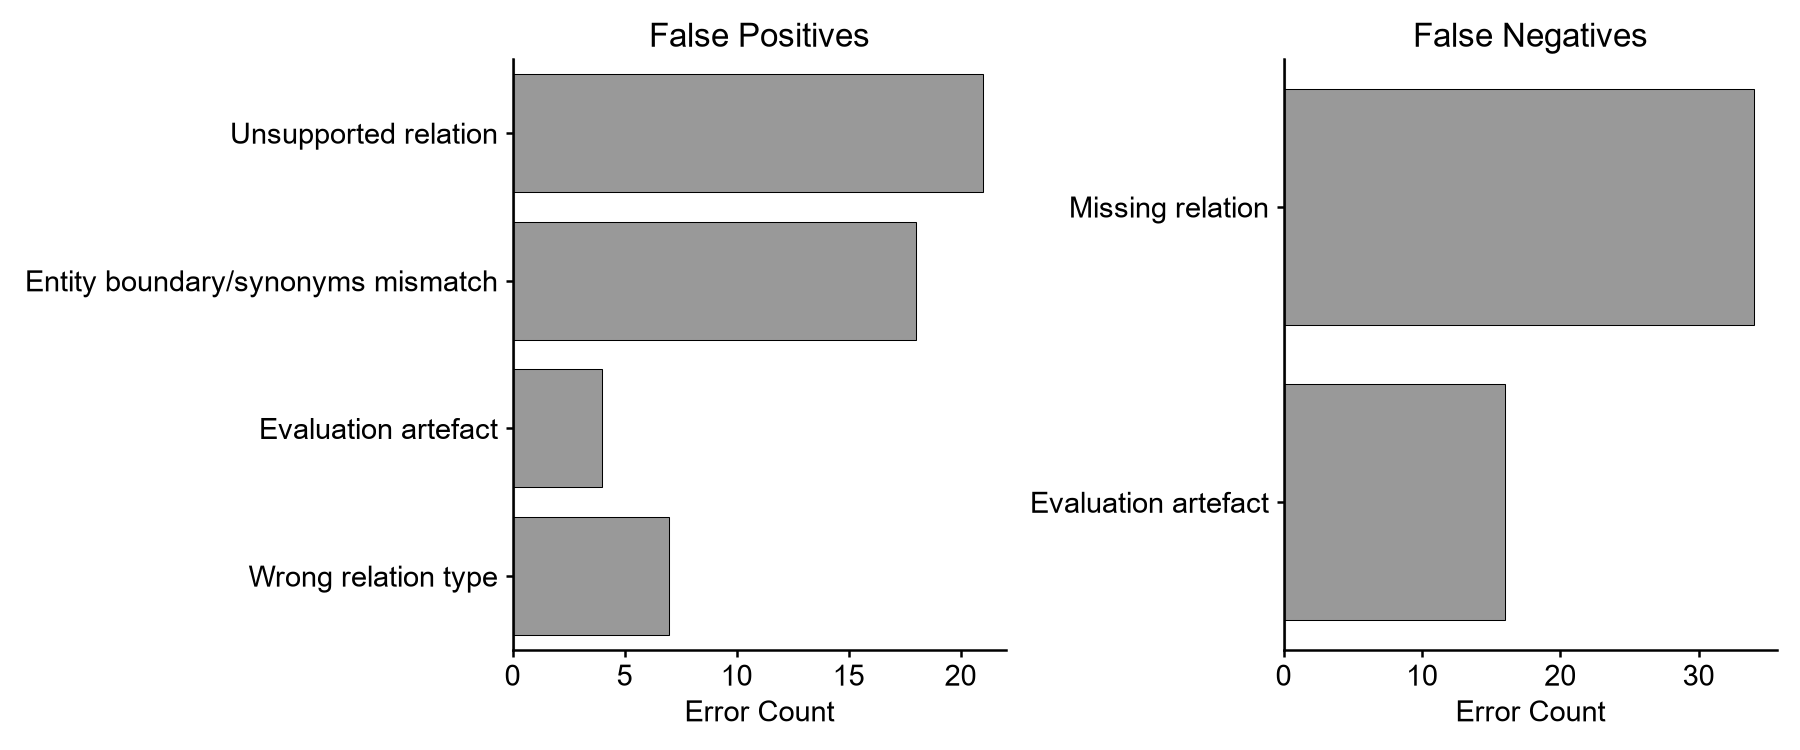
\includegraphics[width=1\textwidth]{../../../img/error_analysis/biored_train/epi_003.png}
    \caption{\texttt{epi\_003} relation error distribution.}
\end{figure}

\begin{figure}[H]
    \centering
    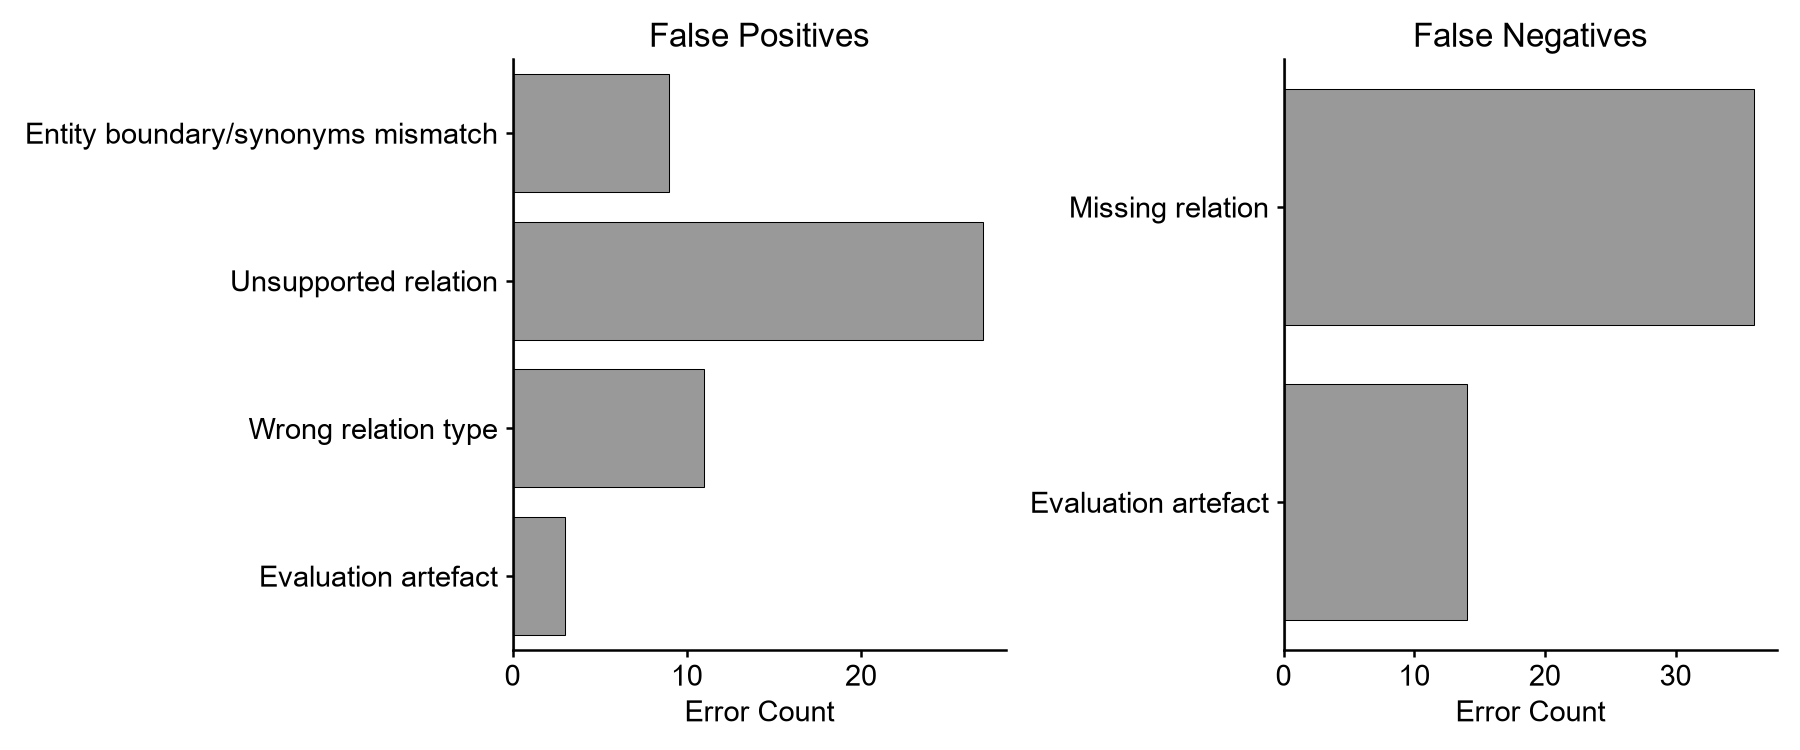
\includegraphics[width=1\textwidth]{../../../img/error_analysis/biored_train/epi_006.png}
    \caption{\texttt{epi\_006} relation error distribution.}
\end{figure}

\begin{figure}[H]
    \centering
    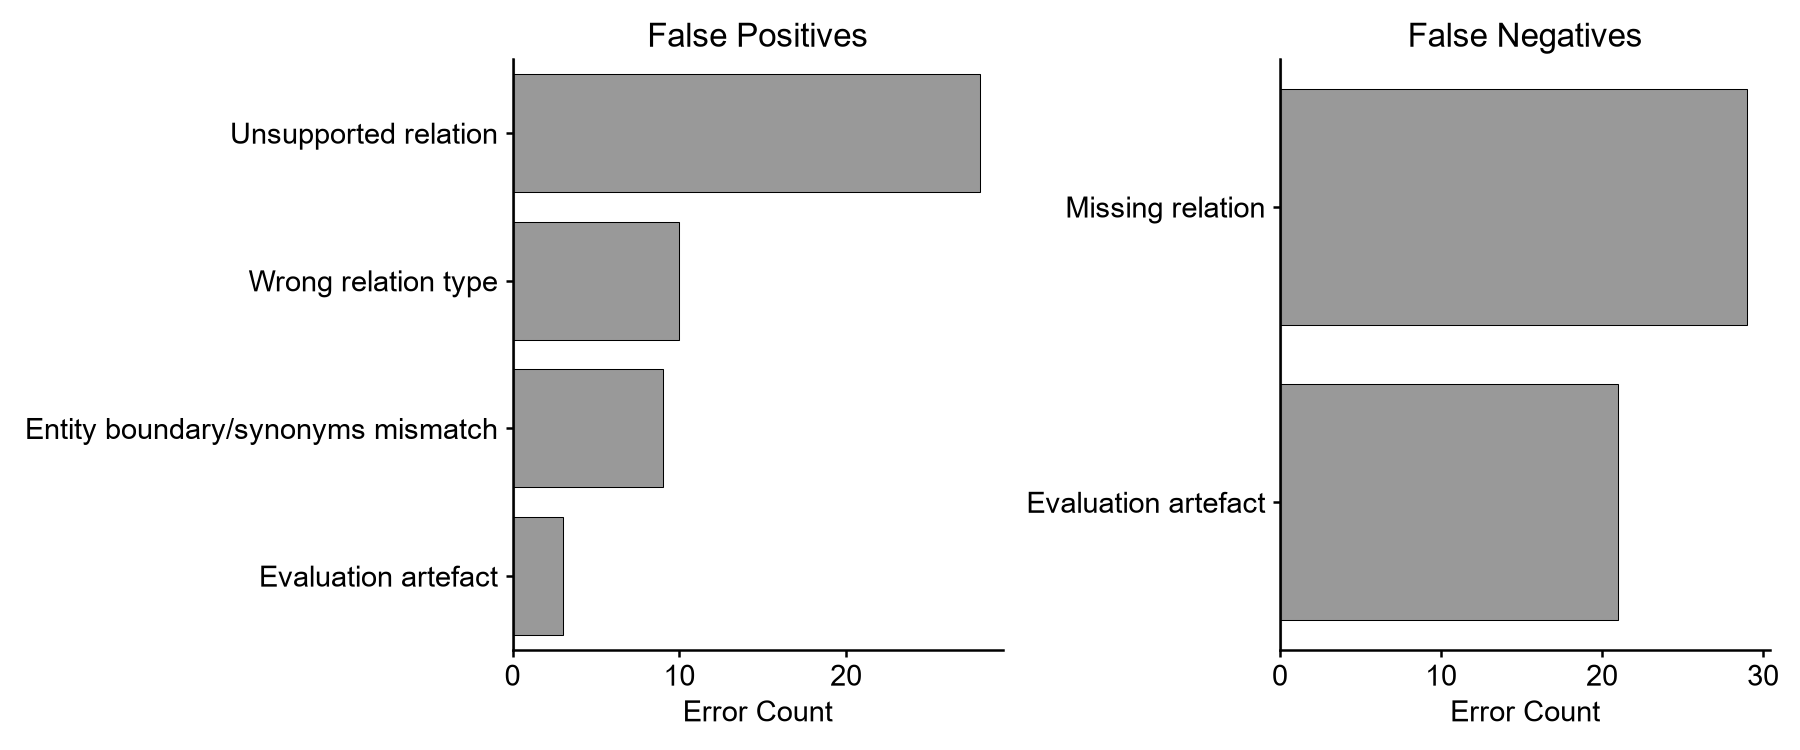
\includegraphics[width=1\textwidth]{../../../img/error_analysis/biored_train/epi_009.png}
    \caption{\texttt{epi\_009} relation error distribution.}
\end{figure}

\begin{figure}[H]
    \centering
    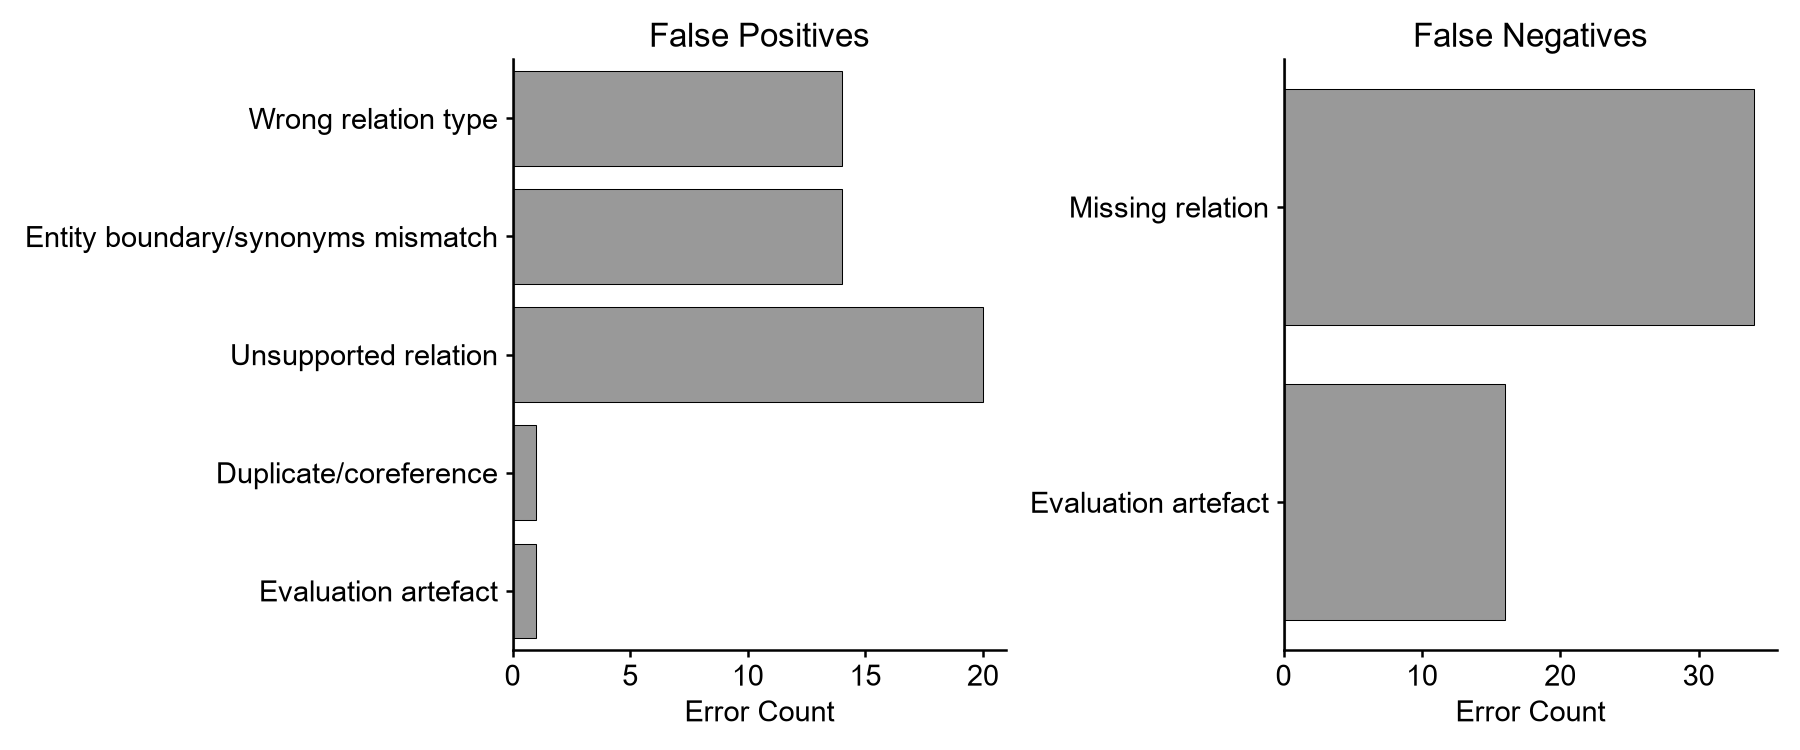
\includegraphics[width=1\textwidth]{../../../img/error_analysis/biored_train/epi_011.png}
    \caption{\texttt{epi\_011} relation error distribution.}
\end{figure}